%
% lines.tex
%
\section{Chart::Lines}
\name{Chart::Lines}
\file{Lines.pm}
\requires{Chart::Base, GD, Carp, FileHandle}
\begin{Description}
\class{Lines} is a subclass of \class{Chart::Base}.\\
The class Lines creates a lines chart.
\end{Description}

\parindent 0pt{\large Example:}


\begin{figure}[h]
	\begin{center}
		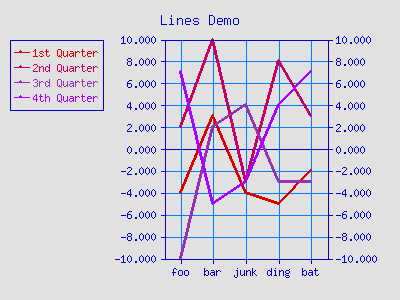
\includegraphics[scale=0.5]{d_lines2.png}
	\end{center}
	\caption{Lines chart}
	\label{fig:lines}
\end{figure}
\begin{verbatim}
use Chart::Lines;

$g = Chart::Lines->new();
$g->add_dataset ('foo', 'bar', 'junk', 'ding', 'bat');
$g->add_dataset ( -4,  3, -4, -5, -2);
$g->add_dataset (  2, 10, -3,  8,  3);
$g->add_dataset (-10,  2,  4, -3, -3);
$g->add_dataset (  7, -5, -3,  4,  7);

%hash = ('legend_labels' => ['1st Quarter', '2nd Quarter',
                             '3rd Quarter', '4th Quarter'],
         'y_axes' => 'both',
         'title' => 'Lines Demo',
         'grid_lines' => 'true',
         'legend' => 'left',
         'legend_example_size' => 20,
         'colors' => {'text' => 'blue',
                      'misc' => 'blue',
                      'background' => 'grey',
                      'grid_lines' => 'light_blue',
                      'dataset0' => [220,0,0],
                      'dataset1' => [200,0,100],
                      'dataset2' => [150,50,175],
                      'dataset3' => [170,0,255] },
         );

$g->set (%hash);

$g->png ("lines.png");
\end{verbatim}

\begin{Constructor} 
An instance of a lines chart object can be created with the constructor \textit{new()}:
\begin{quote}
\fett{\$obj = Chart::Lines->new();}\\
\fett{\$obj = Chart::Lines->new(\parameter{width}, \parameter{height});}
\end{quote}
If \textit{new()} has no arguments, 
the constructor returns an image with the size 300x400 pixels. If new has two arguments
\parameter{width} and \parameter{height}, it returns an image with the desired size.
\end{Constructor}

\Methods
\method{All universal valid methods, see page \pageref{methods} of \class{Chart::Base}.}\\[\parabstand]
%
\Attributes
All universal valid options, see page \pageref{options}. 
Special options for this type of chart are:\\
\begin{description}
\item['y\_axes'] Tells chart where to place the y-axis. 
                 Valid values are 'left', 'right' and 'both'. Defaults to 'left'.

\item['brush\_size'] Sets the width of the lines in pixels. Default is 6.

\item['xy\_plot'] Forces Chart to plot a x-y-graph, which means that the x-axis 
                  is also numeric if set to 'true'. 
                  Very useful for plots of mathematical functions. Defaults to 'false'.

\item['sort'] Sorts the data of a x-y-graph ascending if set to 'true'. 
              Should be set if the added data isn't sorted. Defaults to 'false'.   

\item['stepline'] The points are connected by a stepping function,
                  instead by a direct line if set to 'true'. 
                  Defaults to 'false'.   

\item['stepline\_mode'] Determine whether to start with the first point
                    (if set to 'begin') or end with the last point if set to 'end'.
                    Defaults to 'begin'.   
\end{description}


